\documentclass[12pt, a4paper]{article}

% ============================================================
%  Packages
% ============================================================
\usepackage[utf8]{inputenc}
\usepackage[T1]{fontenc}
\usepackage[english]{babel}
\usepackage{amsmath, amssymb}
\usepackage{geometry}
\usepackage{booktabs}
\usepackage{array}
\usepackage{xcolor}
\usepackage{hyperref}
\usepackage{tikz}
\usetikzlibrary{positioning, arrows.meta, shapes, fit, backgrounds}

\geometry{margin=2.5cm}

\definecolor{depotcolor}{RGB}{220,50,50}
\definecolor{taskcolor}{RGB}{30,100,180}
\definecolor{routeA}{RGB}{52,152,219}
\definecolor{routeB}{RGB}{46,204,113}
\definecolor{routeC}{RGB}{155,89,182}
\definecolor{routeD}{RGB}{230,126,34}
\definecolor{routeE}{RGB}{26,188,156}

\title{Initial Solution Structure in MetaCARP\\
       \large Worked Example on Instance \texttt{gdb1}}
\author{}
\date{}

% ============================================================
\begin{document}
\maketitle
\tableofcontents
\newpage

% ------------------------------------------------------------
\section{Instance \texttt{gdb1} — Overview}
% ------------------------------------------------------------

Instance \texttt{gdb1} is a classical CARP benchmark from the GDB set
(Golden, DeArmon \& Baker, 1983). Its parameters are:

\begin{center}
\renewcommand{\arraystretch}{1.3}
\begin{tabular}{ll}
\toprule
\textbf{Parameter} & \textbf{Value} \\
\midrule
Vertices $|V|$          & 12 \\
Required edges $|R|$    & 22 \\
Vehicles $K$            & 5  \\
Vehicle capacity $Q$    & 5  \\
Depot node              & 1  \\
Best Known Solution (BKS) & 316 \\
\bottomrule
\end{tabular}
\end{center}

% ------------------------------------------------------------
\section{Required Edges (Tasks)}
% ------------------------------------------------------------

Each required edge is a \emph{task}: a street segment that must be
serviced by exactly one vehicle. Tasks are identified by a label
\texttt{TR}$k$ and carry a traversal cost and a demand.
In \texttt{gdb1} all demands equal 1, so a vehicle can serve at most
$Q = 5$ tasks before returning to the depot.

\begin{center}
\renewcommand{\arraystretch}{1.2}
\begin{tabular}{cccc}
\toprule
\textbf{Task} & \textbf{Arc} $(u, v)$ & \textbf{Cost} & \textbf{Demand} \\
\midrule
\texttt{TR1}  & (1, 2)   & 13 & 1 \\
\texttt{TR2}  & (1, 4)   & 17 & 1 \\
\texttt{TR3}  & (1, 7)   & 19 & 1 \\
\texttt{TR4}  & (1, 10)  & 19 & 1 \\
\texttt{TR5}  & (1, 12)  &  4 & 1 \\
\texttt{TR6}  & (2, 3)   & 18 & 1 \\
\texttt{TR7}  & (2, 4)   &  9 & 1 \\
\texttt{TR8}  & (2, 9)   &  2 & 1 \\
\texttt{TR9}  & (3, 4)   & 20 & 1 \\
\texttt{TR10} & (3, 5)   &  5 & 1 \\
\texttt{TR11} & (5, 6)   &  7 & 1 \\
\texttt{TR12} & (5, 11)  & 20 & 1 \\
\texttt{TR13} & (5, 12)  & 11 & 1 \\
\texttt{TR14} & (6, 7)   &  4 & 1 \\
\texttt{TR15} & (6, 12)  &  3 & 1 \\
\texttt{TR16} & (7, 8)   &  8 & 1 \\
\texttt{TR17} & (7, 12)  & 18 & 1 \\
\texttt{TR18} & (8, 10)  &  3 & 1 \\
\texttt{TR19} & (8, 11)  & 10 & 1 \\
\texttt{TR20} & (9, 10)  & 16 & 1 \\
\texttt{TR21} & (9, 11)  & 14 & 1 \\
\texttt{TR22} & (10, 11) & 12 & 1 \\
\bottomrule
\end{tabular}
\end{center}

% ------------------------------------------------------------
\section{Solution Representation}
% ------------------------------------------------------------

A solution $s$ is a list of $K$ routes. Each route is an ordered
sequence of task labels, bracketed by the depot token \texttt{D}
(node 1). Formally:

\[
    s \;=\; \bigl(r_1,\; r_2,\; \ldots,\; r_K\bigr),
    \qquad
    r_k \;=\; (\texttt{D},\; e_1,\; e_2,\; \ldots,\; e_{n_k},\; \texttt{D})
\]

where each $e_i \in R$ is a required edge label and every required
edge appears in exactly one route (coverage constraint).

\subsection{Feasibility constraints}

\begin{itemize}
    \item \textbf{C1 — Coverage:} every task $e \in R$ is served by
          exactly one vehicle.
    \item \textbf{C2 — Route structure:} each route starts and ends
          at the depot.
    \item \textbf{C3 — Capacity:} $\sum_{e \in r_k} d(e) \leq Q$
          for every route $r_k$.
\end{itemize}

When C3 is violated, a penalty term $\lambda \cdot \phi(s)$ is added
to the objective, where $\phi(s) = \sum_k \max(0,\,\sum_{e \in r_k} d(e) - Q)$.

\subsection{In-memory Python representation}

Internally the solution is stored as a \texttt{list[list[str]]}:

\begin{verbatim}
s = [
    ['D', 'TR1',  'TR6',  'TR9',  'TR20', 'TR22', 'D'],   # route 1
    ['D', 'TR2',  'TR7',  'TR8',  'TR21', 'TR19', 'D'],   # route 2
    ['D', 'TR3',  'TR14', 'TR11', 'TR12', 'D'],            # route 3
    ['D', 'TR4',  'TR18', 'TR16', 'TR17', 'D'],            # route 4
    ['D', 'TR5',  'TR13', 'TR10', 'TR15', 'D'],            # route 5
]
\end{verbatim}

For fast vectorized evaluation inside the metaheuristic loops, the
\texttt{D} tokens are stripped and each task label is mapped to an
integer ID via a \texttt{SearchEncoding} lookup table, producing a
\texttt{list[list[int]]} representation.

% ------------------------------------------------------------
\section{Initial Solution for \texttt{gdb1}}
% ------------------------------------------------------------

The table below shows the five routes of the initial solution loaded
from the pre-computed pickle file, together with the accumulated
demand per route and the feasibility check against $Q = 5$.

\begin{center}
\renewcommand{\arraystretch}{1.4}
\begin{tabular}{clcc}
\toprule
\textbf{Route} & \textbf{Tasks (sequence)} & \textbf{Demand} & \textbf{Feasible?} \\
\midrule
$r_1$ & \texttt{TR1 $\to$ TR6 $\to$ TR9 $\to$ TR20 $\to$ TR22}
      & $1+1+1+1+1 = 5$ & \checkmark \\
$r_2$ & \texttt{TR2 $\to$ TR7 $\to$ TR8 $\to$ TR21 $\to$ TR19}
      & $1+1+1+1+1 = 5$ & \checkmark \\
$r_3$ & \texttt{TR3 $\to$ TR14 $\to$ TR11 $\to$ TR12}
      & $1+1+1+1 = 4$   & \checkmark \\
$r_4$ & \texttt{TR4 $\to$ TR18 $\to$ TR16 $\to$ TR17}
      & $1+1+1+1 = 4$   & \checkmark \\
$r_5$ & \texttt{TR5 $\to$ TR13 $\to$ TR10 $\to$ TR15}
      & $1+1+1+1 = 4$   & \checkmark \\
\midrule
\multicolumn{2}{r}{\textbf{Total tasks covered}} & 22 & \checkmark \\
\bottomrule
\end{tabular}
\end{center}

All 22 tasks are covered, all demands satisfy $Q = 5$, and each route
starts and ends at depot node 1. The initial solution is therefore
\textbf{fully feasible}.

% ------------------------------------------------------------
\section{Visual Route Diagram}
% ------------------------------------------------------------

The diagram below represents each route as a sequence of boxes.
The depot \texttt{D} (node 1) is shown in red at the start and end of
every route. Each task box shows its label and the arc it covers.

\vspace{1em}
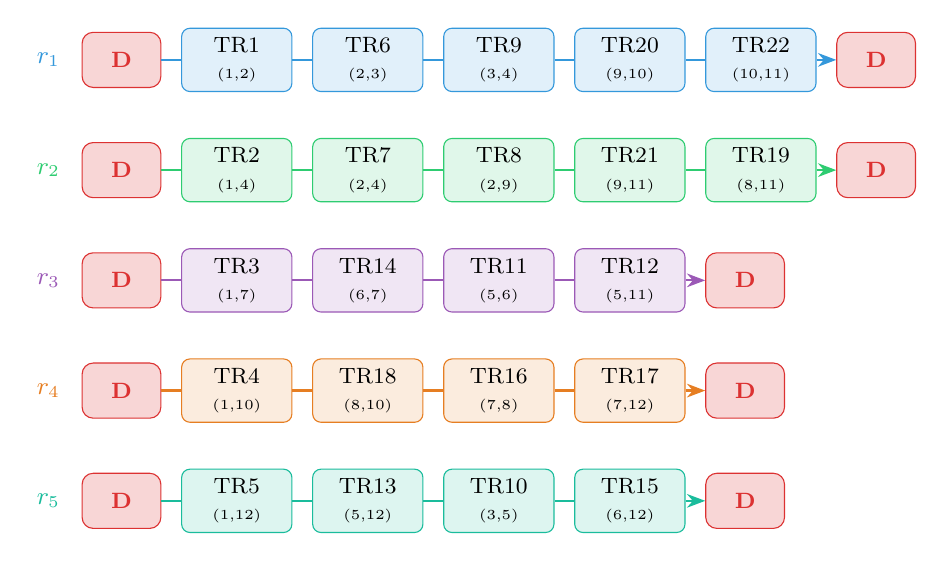
\begin{tikzpicture}[
    depot/.style={draw=depotcolor, fill=depotcolor!20, rounded corners=4pt,
                  minimum width=1cm, minimum height=0.7cm, font=\footnotesize\bfseries},
    task/.style={draw=#1, fill=#1!15, rounded corners=3pt,
                 minimum width=1.4cm, minimum height=0.7cm, font=\footnotesize},
    arr/.style={->, >=Stealth, thick},
    every node/.style={align=center}
]

% ---- Route 1 ----
\node[depot]  (d1s) at (0, 0)   {\textcolor{depotcolor}{D}};
\node[task=routeA, right=0.25cm of d1s]  (r1t1) {TR1\\{\tiny(1,2)}};
\node[task=routeA, right=0.25cm of r1t1] (r1t2) {TR6\\{\tiny(2,3)}};
\node[task=routeA, right=0.25cm of r1t2] (r1t3) {TR9\\{\tiny(3,4)}};
\node[task=routeA, right=0.25cm of r1t3] (r1t4) {TR20\\{\tiny(9,10)}};
\node[task=routeA, right=0.25cm of r1t4] (r1t5) {TR22\\{\tiny(10,11)}};
\node[depot, right=0.25cm of r1t5]       (d1e)  {\textcolor{depotcolor}{D}};
\node[left=0.15cm of d1s, font=\small\bfseries, text=routeA] {$r_1$};
\draw[arr, color=routeA] (d1s)--(r1t1)--(r1t2)--(r1t3)--(r1t4)--(r1t5)--(d1e);

% ---- Route 2 ----
\node[depot]  (d2s) at (0,-1.4) {\textcolor{depotcolor}{D}};
\node[task=routeB, right=0.25cm of d2s]  (r2t1) {TR2\\{\tiny(1,4)}};
\node[task=routeB, right=0.25cm of r2t1] (r2t2) {TR7\\{\tiny(2,4)}};
\node[task=routeB, right=0.25cm of r2t2] (r2t3) {TR8\\{\tiny(2,9)}};
\node[task=routeB, right=0.25cm of r2t3] (r2t4) {TR21\\{\tiny(9,11)}};
\node[task=routeB, right=0.25cm of r2t4] (r2t5) {TR19\\{\tiny(8,11)}};
\node[depot, right=0.25cm of r2t5]       (d2e)  {\textcolor{depotcolor}{D}};
\node[left=0.15cm of d2s, font=\small\bfseries, text=routeB] {$r_2$};
\draw[arr, color=routeB] (d2s)--(r2t1)--(r2t2)--(r2t3)--(r2t4)--(r2t5)--(d2e);

% ---- Route 3 ----
\node[depot]  (d3s) at (0,-2.8) {\textcolor{depotcolor}{D}};
\node[task=routeC, right=0.25cm of d3s]  (r3t1) {TR3\\{\tiny(1,7)}};
\node[task=routeC, right=0.25cm of r3t1] (r3t2) {TR14\\{\tiny(6,7)}};
\node[task=routeC, right=0.25cm of r3t2] (r3t3) {TR11\\{\tiny(5,6)}};
\node[task=routeC, right=0.25cm of r3t3] (r3t4) {TR12\\{\tiny(5,11)}};
\node[depot, right=0.25cm of r3t4]       (d3e)  {\textcolor{depotcolor}{D}};
\node[left=0.15cm of d3s, font=\small\bfseries, text=routeC] {$r_3$};
\draw[arr, color=routeC] (d3s)--(r3t1)--(r3t2)--(r3t3)--(r3t4)--(d3e);

% ---- Route 4 ----
\node[depot]  (d4s) at (0,-4.2) {\textcolor{depotcolor}{D}};
\node[task=routeD, right=0.25cm of d4s]  (r4t1) {TR4\\{\tiny(1,10)}};
\node[task=routeD, right=0.25cm of r4t1] (r4t2) {TR18\\{\tiny(8,10)}};
\node[task=routeD, right=0.25cm of r4t2] (r4t3) {TR16\\{\tiny(7,8)}};
\node[task=routeD, right=0.25cm of r4t3] (r4t4) {TR17\\{\tiny(7,12)}};
\node[depot, right=0.25cm of r4t4]       (d4e)  {\textcolor{depotcolor}{D}};
\node[left=0.15cm of d4s, font=\small\bfseries, text=routeD] {$r_4$};
\draw[arr, color=routeD] (d4s)--(r4t1)--(r4t2)--(r4t3)--(r4t4)--(d4e);

% ---- Route 5 ----
\node[depot]  (d5s) at (0,-5.6) {\textcolor{depotcolor}{D}};
\node[task=routeE, right=0.25cm of d5s]  (r5t1) {TR5\\{\tiny(1,12)}};
\node[task=routeE, right=0.25cm of r5t1] (r5t2) {TR13\\{\tiny(5,12)}};
\node[task=routeE, right=0.25cm of r5t2] (r5t3) {TR10\\{\tiny(3,5)}};
\node[task=routeE, right=0.25cm of r5t3] (r5t4) {TR15\\{\tiny(6,12)}};
\node[depot, right=0.25cm of r5t4]       (d5e)  {\textcolor{depotcolor}{D}};
\node[left=0.15cm of d5s, font=\small\bfseries, text=routeE] {$r_5$};
\draw[arr, color=routeE] (d5s)--(r5t1)--(r5t2)--(r5t3)--(r5t4)--(d5e);

\end{tikzpicture}

\vspace{1em}
Each arrow represents vehicle movement: \textbf{service} when traversing
a task arc, or \textbf{deadheading} (empty travel) when repositioning
between consecutive tasks. Deadheading cost is computed via shortest
paths on $G$ and is included in the total route cost.

% ------------------------------------------------------------
\section{Cost Evaluation}
% ------------------------------------------------------------

The total cost of a solution is the sum of:
\begin{enumerate}
    \item \textbf{Service cost:} the traversal cost of each required edge.
    \item \textbf{Deadheading cost:} the shortest-path cost of every
          empty repositioning between consecutive tasks and the return
          to the depot.
\end{enumerate}

Formally, for vehicle $k$ with route
$r_k = (e_1, e_2, \ldots, e_{n_k})$:

\[
    \text{cost}(r_k) \;=\;
    d_{\text{SP}}(\text{depot},\; u_{e_1})
    \;+\; \sum_{i=1}^{n_k} c(e_i)
    \;+\; \sum_{i=1}^{n_k - 1} d_{\text{SP}}(v_{e_i},\; u_{e_{i+1}})
    \;+\; d_{\text{SP}}(v_{e_{n_k}},\; \text{depot})
\]

where $u_e$ and $v_e$ are the start and end nodes of arc $e$,
$c(e)$ is its traversal cost, and $d_{\text{SP}}(\cdot,\cdot)$ is the
shortest-path distance precomputed via Dijkstra.

The total solution cost is $\text{cost}(s) = \sum_{k=1}^{K} \text{cost}(r_k)$.

\subsection{Penalized objective}

During metaheuristic search, infeasible solutions (violating C3) are
allowed but penalized:

\[
    f(s) \;=\; \text{cost}(s) \;+\; \lambda \cdot \phi(s),
    \qquad
    \phi(s) = \sum_{k=1}^{K} \max\!\Bigl(0,\; \textstyle\sum_{e \in r_k} d(e) - Q\Bigr)
\]

The penalty coefficient $\lambda$ is set automatically by
$\lambda_{\text{default}}$ based on the instance's average arc cost
and average demand, ensuring that a single unit of excess demand is
penalized more than the average arc cost.

\end{document}
